\subsection{Backend}
\label{sub:backend}
  Da der GTFS Standard eine fertige relationale Beziehung der einzelnen Dateien festlegt, ist der Einsatz einer relationalen Datenbank sehr naheliegend. Dabei gibt es eine breite Palette an Auswahl. Damit die Anwendung möglichst Zugänglich bleibt, liegt der Fokus auf Datenbanken die unter einer Open-source Lizenz kostenfrei zur Verfügung stehen. Die zwei populärsten sind MySQL und PostgreSQL\parencite{db_engines}. Beide haben ihre Vor- und Nachteile und die Entscheidung ist mehr eine persönliche Präferenz, als ein großer Vorteil des Einen über den Anderen. Einen kleinen Vorteil bietet PostgreSQL's Unterstützung für Array-Types, welche sehr hilfreich beim speichern und abfragen von Daten ist. Ansonsten ist dieses Projekt auch mit MySQL realisierbar.\\

  In diesem Abschnitt soll beschrieben werden, welche Probleme beim Arbeiten mit dem GTFS Datenformat und einer PostgreSQL Datenbank bestehen und wie diese gelöst wurden. Dabei steht vor allem die Behebung von Engpässen bei der Query\footnotemark Performance, als auch die Verringerung der zu verarbeitenden Datenmenge.

  \footnotetext{Ein Query ist eine Informationsanfrage an eine Datenbank} 
  
  % Gliederung eventuell nochmals beschreiben.

  \subsubsection{GTFS - Probleme und Herausforderungen}
\label{ssub:gtfs_probleme_und_herausforderungen}
   Bereits 1993 stellte \texttt{Jakob Nielsen} einen Richtwert für die Antwortzeit einer schnellen Webanwendung vor:

  \begin{quote}
    \textit{"`1.0 second is about the limit for the user's flow of thought to stay uninterrupted, even though the user will notice the delay. Normally, no special feedback is necessary during delays of more than 0.1 but less than 1.0 second, but the user does lose the feeling of operating directly on the data."'}\parencite{nielsen}
  \end{quote}

  Ob oder wie dies Antwortzeit erreicht werden kann, soll hier nicht vertieft werden, denn zu diesem Thema habe ich bereits meine Bachelorarbeit gewidmet\parencite{lorer}.

  Damit eine Webanwendung aber überhaupt eine Chance hat, diese Geschwindigkeitsmarke zu erreichen, ist eine schnelle Antwortzeit des Backends sehr wichtig. Dabei sind Antwortzeiten Innerhalb von 0 bis 200 Millisekunden ein sehr guter Wert. Natürlich gilt: Je weniger umso besser. Diese Benchmark mit dem GTFS Format zu erreichen war eine der Hauptherausforderungen dieser Arbeit.\\

  Das GTFS Format hat den entscheidenden Nachteil, dass es eine hohe Komplexität aufweist, sobald Daten aus verschiedenen Tabellen benötigt werden. Für eine Live Visualisierung, sind Daten aus nahezu allen Tabellen relevant. Abbildung~\ref{fig:gtfs_joined_tables} zeigt, welche davon benötigt - beziehungsweise nicht benötigt werden (grau).

  \begin{figure}[ht]
    \begin{center}
      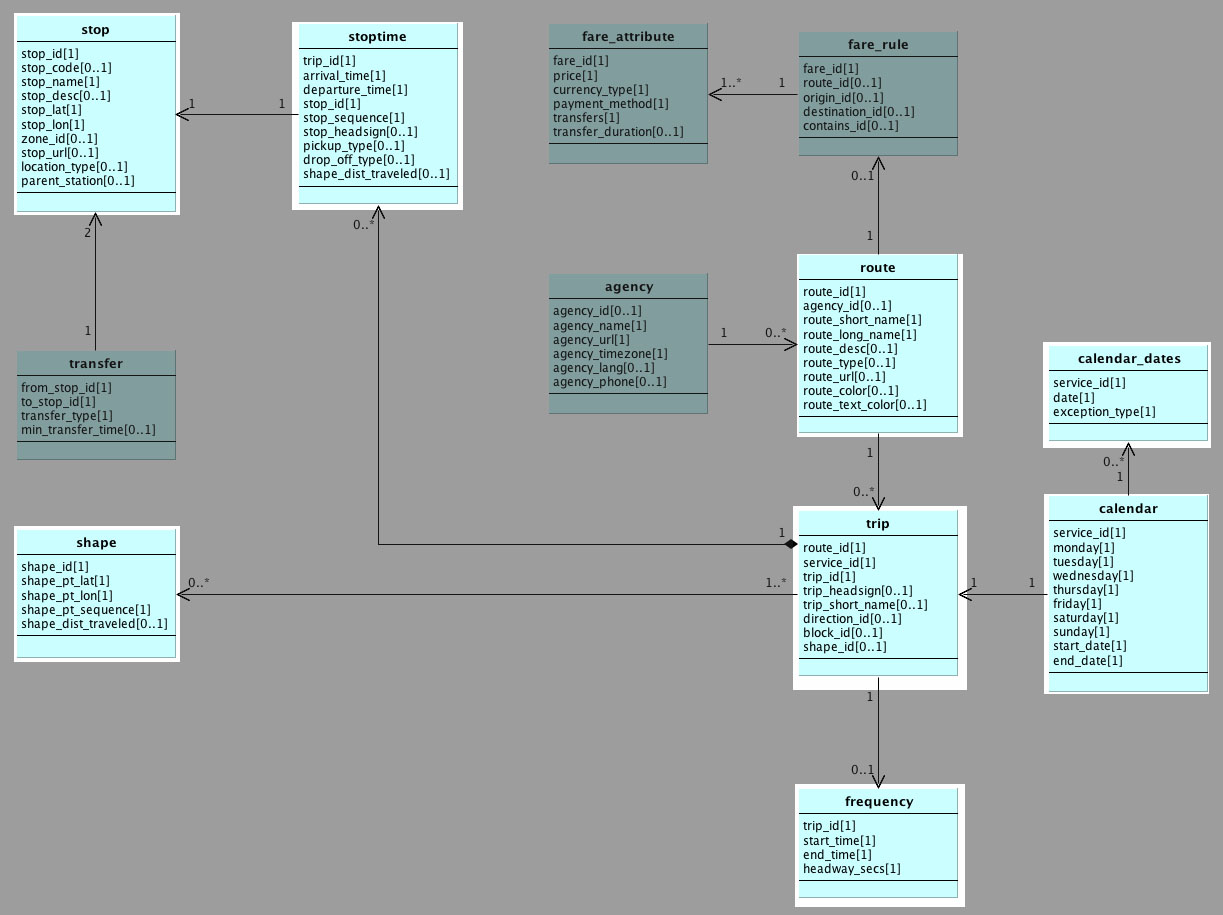
\includegraphics[width=\textwidth]{gtfs_joined_tables.jpg}
      \caption{Benötigte GTFS Tabellen\parencite{google_gtfs_reference}}
      \label{fig:gtfs_joined_tables}
    \end{center}
  \end{figure}

  Das UML Diagramm ist auf den ersten Blick relativ simpel zu verstehen und die Grundlagen der verschiedenen Relationen wurde bereits in Kapitel~\ref{ssec:gtfs_datenformat} beschrieben. Wo liegt also das Problem? In Worten ließe sich diese Datenbankabfrage mit folgendem Statement beschreiben: 

  \begin{quote}
    \label{query_statement}
    \textit{"`Gib uns alle aktiven Trips mit deren Linienverlauf, die am heutigen Tag aktiv sind und in einer Zeitspanne zwischen $t_a$ und $t_b$ liegen."'}
  \end{quote}

  Das große Problem dieses Satze liegt in der Zeitkomponente \textit{"`Trips die am heutigen Tag aktiv sind zwischen ..."'}. Die Trip Tabelle selbst (bezogen auf Abbildung~\ref{fig:gtfs_joined_tables}), hat dies bezüglich keinerlei Informationen darüber. Auch die Calendar- und Calendar-Dates Tabelle beinhaltet nur Informationen, an welchem Datum ein Trip stattfindet, nicht aber um welche Uhrzeit. 

  Erst die Stoptime Tabelle ermöglicht es uns, eine Aussage zu treffen, wann ein Trip aktiv ist. Über die zwei Felder \texttt{arrival\_time} und \texttt{departure\_time} lässt sich sagen, zu welchem Zeitpunkt ein Vehicle an einer Station anhält. Die erste und letzte Station ($S_1$ und $S_n$) geben uns also einen zeitlichen Rahmen, in dem der Trip aktiv ist.
  Hierbei wird klar, dass allein die Beantwortung der Frage zur zeitlichen Komponente, bereits sehr viele Daten aus verschiedenen Tabellen benötigt. Die anderen Tabellen wie \texttt{shape}, \texttt{route}, \texttt{stop} und \texttt{frequency} würden für weitere Informationen wie Vehicle Farbe, Stop Position (Längen- und Breitengrad) oder den Linienverlauf (shape) benötigt werden. Um an die Daten zu gelangen, müssen alle benötigten Tabellen mittels SQL \texttt{JOIN} miteinander verknüpft werden. Dies geschieht durch die Verbindung der einzelnen Reihen zweier Tabellen (TabelleA und TabelleB) gegen eine Verknüpfungsbedingung. Das Resultat ist eine neue Ergebnistabelle mit den Inhalten der kombinierten Reihen. Solche Verknüpfungen sind besonders dann Zeitintensiv, wenn eine große Menge an Daten (siehe Tabelle:~\ref{table:table_metrics}) kombiniert werden. Die Metriken der Tabellen sind dabei wie folgt:

  \begin{longtable}{|>{\raggedright \arraybackslash}p{5.0cm}|>{\raggedright \arraybackslash}p{5.0cm}|>{\raggedright \arraybackslash}p{5.0cm}|}
  \caption{Tabellen Metriken} \label{table:table_metrics}\\
    \hline
    Tabellen Name & Anzahl Reihen\\
    \hline
    trips.txt & 71,000\\
    stop\_times.txt & 1,3000,000\\
    stops.txt & 7,900\\
    shapes.txt & 1,085,860\\
    \hline
  \end{longtable}
  
  Die für das oben genannte Statement~\ref{query_statement} äquivalente SQL-Abfrage ist aufgrund seiner Länge (113 Zeilen Code) im Anhang unter Listing~\ref{lst:get_active_trips_query} zu finden. Diese SQL Abfrage ist allerdings nicht Performant. Sollen alle Trips in einem Zeitraum von 1 - 15 Minuten gefunden werden, sind bereits Rechenzeiten entstanden, die aufgrund ihrer langen Laufzeit abgebrochen werden mussten. In mehreren Iterationen wurde versucht die SQL-Abfrage zu optimieren, was allerdings keine Verbesserung herbeiführte. Es sind zu viele JOIN Verknüpfungen und WHERE Bedingungen in dieser Abfrage, als das sich eine Performante Lösung damit finden lässt. Es musste ein neuer Ansatz gefunden werden um Abfragezeiten erheblich zu verringern.
  
% subsubsection gtfs_probleme_und_herausforderungen (end)
  \subsubsection{GTFS Optimierungen}
\label{ssub:gtfs_optimierungen}

  Der erste Schritt um die Performance zu verbessern, ist die Optimierung von GTFS Feeds. Damit lässt sich die Datenmenge bereits vor dem Importieren in die Datenbank, erheblich verringern. Ein Tool um ein GTFS Feed umfassend zu optimieren ist \texttt{gtfstidy} \url{https://github.com/patrickbr/gtfstidy}. Es bietet dabei allerdings nicht nur die Möglichkeit für die Vereinfachung von Polylines sondern kommt mit einer ganzen Reihe an Optimierungsmöglichkeiten. 

  Der Kommandozeilenbefehl \colorbox{materialGrey}{\texttt{\color{white}{\$ gtfstidy -sSiRDeO input.zip output}}} optimiert das Stuttgart-VVS Feed wie folgt:
  
  \begin{itemize}[label={}]
    \item \textbf{-s} Reduziert die Punktanzahl einer Polyline
      
    \item \textbf{-S} Entfernt redundante Polylines.

    \item \textbf{-i} Umwandlung von Zeichen ID's (String) in Zahlen ID's (Integer).\footnote{Aus der String ID \texttt{'1.T0.10-1-j17-1.16.H'} wird \texttt{78}}

    \item \textbf{-O} Entfernt Feed Einträge die nicht referenziert werden.

    \item \textbf{-R} Entfernt doppelt vorhandene Routen.

    \item \textbf{-e} Setzt fehlerhafte oder optionale Felder auf einen Standard Wert.

    \item \textbf{-D} Entfernt fehlerhafte Einträge aus dem Feed.
  \end{itemize}

  Durch Verwendung von gtfstidy konnte das Feed optimiert werden und die Datengröße der einzelnen Dateien um folgendes Maß verringert werden.

  \begin{longtable}{|>{\raggedright \arraybackslash}p{5.0cm}|>{\raggedright \arraybackslash}p{5.0cm}|>{\raggedright \arraybackslash}p{5.0cm}|}
    \hline
    Dateiname & Größe davor& Größe danach\\
    \hline
    trips.txt & 6 MB & 2.8 MB\\
    stop\_times.txt & 103 MB & 53 MB\\
    stops.txt & 651 KB & 355 KB\\
    shapes.txt & 77.3 MB & 22.4 MB\\
    routes.txt & 54 KB & 38 KB\\
    calendar\_dates.txt & 557 KB & 463 KB\\
    \hline
    \caption{Tabellengröße bevor und nach anwenden von gtfstidy}
    \label{tbl:gtfs_tidy_results}
  \end{longtable}

  Insgesamt konnte so die Größe des Feeds von 79 MB auf 118 MB um knapp 50\% verringert werden. Vor allem die Umwandlung von langen String ID's in kürzere Integer ID's trägt maßgeblich zur Verringerung der Dateigröße bei.

% subsubsection gtfs_optimierungen (end)
  \subsubsection{Polyline optimieren}
\label{ssub:polyline_optimieren}

  Die Optimierung der Polyline ist ein sehr wichtiger Aspekt in meiner Arbeit und soll in diesem Abschnitt vertieft werden.

  \subsubsection*{Ramer–Douglas–Peucker}
  \label{ssub:ramer_douglas_peucker}
    Das Problem: Die im Stuttgart-VVS Feed zur Verfügung gestellten Polylines sind Überdefiniert und können aus tausenden Punkten bestehen. Für eine Visualisierung ist eine solche Genauigkeit nicht notwendig und aufgrund der großen Datenmenge problematisch. Im vorigen Abschnitt \ref{ssub:gtfs_optimierungen} wurde die Option \colorbox{materialGrey}{\texttt{\color{white}{-s}}} vorgestellt. Dieser Befehl verwendet den "`Ramer–Douglas–Peucker"' (RDP) Algorithmus um die Anzahl der Punkte einer Polyline zu reduzieren. Der Vorteil besteht darin, dass dabei nicht der Linienverlauf verändert wird. Abbildung~\ref{fig:simplify} zeigt ein Beispiel einer solchen Vereinfachung mittels einer JavaScript Bibliothek\footnote{Simplify.js \url{http://mourner.github.io/simplify-js/}}.

    \begin{figure}[htbp]
      \centering
      \subfloat[Polyline vor RDP]{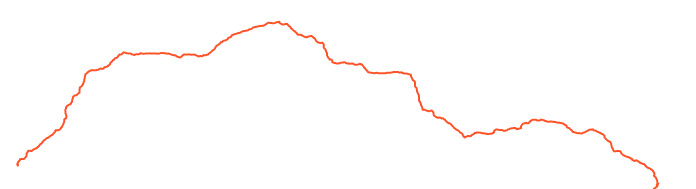
\includegraphics[width=0.48\textwidth]{simplify_before.jpg}\label{fig:simplify_before}}
      \hfill
      \subfloat[Polyline nach RDP]{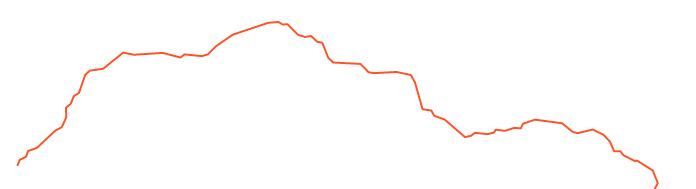
\includegraphics[width=0.48\textwidth]{simplify_after.jpg}\label{fig:simplify_after}}
      \caption{Vereinfachung einer Polyline mittels Simplify.js}
      \label{fig:simplify}
    \end{figure}

    Ausgangspunkt ist eine Polyline mit $\approx1000$ Punkten (\ref{fig:simplify}a). Nach der Vereinfachung (\ref{fig:simplify}b) ist die Anzahl auf 100 Punkte reduziert, ohne dabei visuell merklich einzubüßen. Dies ist eine erhebliche Reduzierung der Punkte um 90\%. Wie wirkt sich dieser Algorithmus positiv auf das Projekt aus? Die Vorteile sind weitreichend. Sehen wir uns die Shape Tabelle in Abbildung \ref{fig:shape_simplify} an. \ref{fig:shape_simplify}a zeigt 394 Reihen vor der Optimierung und nur noch 140 (\ref{fig:shape_simplify}b) nach Anwendung von gtfstidy.

    \begin{figure}[htbp]
      \centering
      \subfloat[Shapte Tabelle vor RDP]{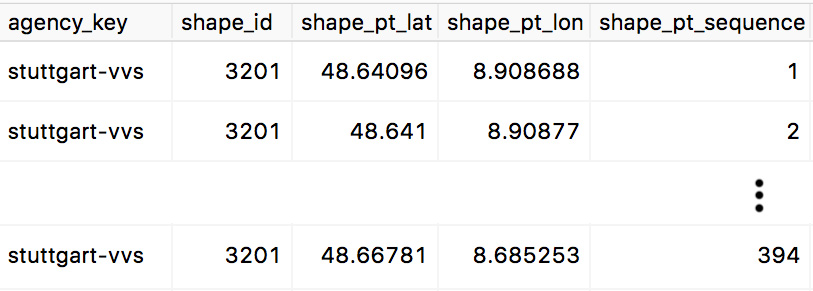
\includegraphics[width=0.48\textwidth]{shape_simplify_before.jpg}\label{fig:shape_simplify_before}}
      \hfill
      \subfloat[Shapte Tabelle nach RDP]{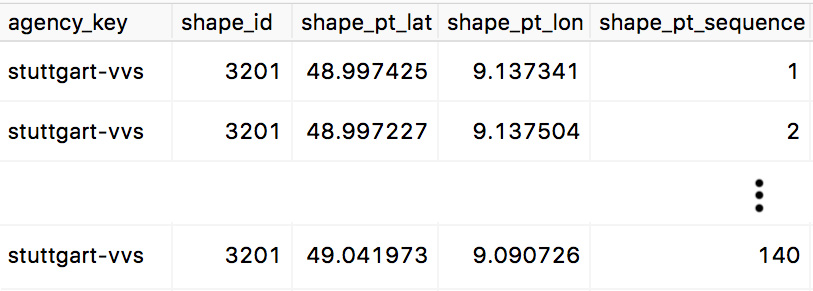
\includegraphics[width=0.48\textwidth]{shape_simplify_after.jpg}\label{fig:shape_simplify_after}}
      \caption{Reduzieren der Polyline via gtfstidy}
      \label{fig:shape_simplify}
    \end{figure}

    In seinem Originalzustand hat das verwendete VVS Feed 1,085,859 Mio Zeilen. Nach der Anwendung sind diese auf 617,653 Tsd. verringert. Testet man folgende PostgreSQL Abfrage
    \colorbox{materialGrey}{\texttt{\color{white}{{\color{materialBlue}SELECT} * {\color{materialBlue}FROM} gtfs\_shapes {\color{materialBlue}WHERE} shape\_id = {\color{materialRed}3201}}}}
    die alle Punkte einer Polyline ausgeben soll, so ergibt sich für ein optimiertes Feed eine Query Zeit von $\approx145 ms$ und für das nicht optimierte Feed $\approx250 ms$. Schon durch diese einfache Methode sind bereits erste Performance Steigerungen wahrnehmbar.

  % subsubsection ramer_douglas_peucker (end)

  \subsubsection*{Aggregieren der Shape Tabelle}
  \label{ssub:aggregieren_der_shape_tabelle}
    In GTFS wird für jeden Punkt einer Polyline eine Reihe in der Datenbank belegt. Diese Abfolge ist durch eine sogenannte \texttt{Shape Point Sequence} festgelegt, was nichts anderes ist als eine Zahl von $1$ bis $n$. Dies ist auch bereits in obiger Tabelle \ref{fig:shape_simplify} zu sehen gewesen. Sehr viel effektiver wäre es allerdings, diese Punkte nicht Reihenweise zu speichern, sondern alle zusammen gehörenden Punkte in einem einzigen Feld zu speichern. Dies ist in PostgreSQL durch eine Aggregierung möglich. Daraus ergibt sich folgende Shape Tabelle:

    \begin{figure}[htbp]
      \begin{center}
        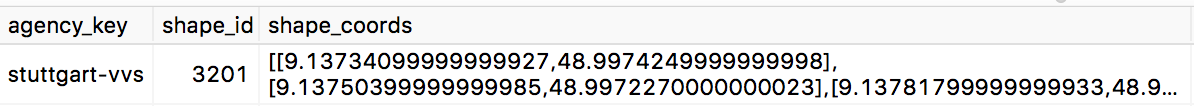
\includegraphics[width=\textwidth]{aggregated.png}
        \caption{Aggregierte Koordinaten der Shape Tabelle}
        \label{fig:aggregated}
      \end{center}
    \end{figure}

    Wie zu sehen ist benötigt nun eine Polyline in der Shape Tabelle nicht mehr 140 Reihen, sondern nur noch eine einzige. Für diese Arbeit ist dies auf alle Polylines angewendet worden und in einer neuen Tabelle namens \texttt{denormalized\_shapes} abgespeichert. Dadurch ist die Berechnung der Aggregierung nur einmal nötig. Der SQL-Befehl dafür ist dem Anhang unter \ref{lst:sql_aggregate_shape}. zu entnehmen.
    Wenden wir die selbe SQL Abfrage, die bereits oben Verwendung fand, auf die neue \texttt{denormalized\_shapes} Tabelle an. Die Query Zeit ist auf $\approx1ms$ gesunken! Anstatt hunderte Reihen muss nur eine einzige Reihe ausgelesen werden, was sehr sehr schnell ist. Durch das Denormalisieren\footnotemark der Shape Tabelle ist auch die Anzahl der Reihen auf ein Minimum gesunken. Von den früheren 617,653 Tsd. Reihen, sind jetzt durch die Aggregation nur noch 4,524 Tsd. übrig.

    \footnotetext{Denormalisieren beschreibt den Prozess der Relationsauflösung von Datenbanktabellen.}
  
  % subsubsection aggregieren_der_shape_tabelle (end)

  \subsubsection*{Polyline Encoding}
  \label{ssub:polyline_encoding}
    Die letzte Maßnahme zur Optimierung der Polyline stellt das sogenannte Polyline Encoding dar. Wie dieses Verfahren genau funktioniert, geht an dieser Stelle zu weit. Hier soll nur erklärt werden, was das Polyline Encoding für diese Arbeit bedeutet und warum es verwendet wird.\\

    Das Polyline Encoding kann in JavaScript beispielsweise durch das Google-Polyline\footnote{\url{https://www.npmjs.com/package/google-polyline}} Paket eingesetzt werden. Das Encoding wandelt eine Polyline, bestehend aus Punkten, in einen String um. Zum Beispiel die Punkte: (38.5, -120.2), (40.7, -120.95), (43.252, -126.453) werden als
    \colorbox{materialGrey}{\texttt{\color{white}{\_p\textasciitilde iF\textasciitilde ps|U\_ulLnnqC\_mqNvxq`@}}}
    codiert. Dies geschieht in meiner Anwendung immer genau dann, bevor Daten von Server in Richtung Client geschickt werden: Encode $\rightarrow$ Send $\rightarrow$ Decode. Da eine codierte Polyline weniger Zeichen benötigt, kann damit Datenvolumen bei der Kommunikation zwischen Server und Client gespart werden.

  % subsubsection polyline_encoding (end)


% subsubsection polyline_optimieren (end)
  \subsubsection{Erstellen der Datenbank}
\label{ssub:erstellen_der_datenbank}
  init.sh
% subsubsection erstellen_der_datenbank (end)
  \subsubsection{Daten importieren}
\label{sub:daten_importieren}
  import.sh
% subsubsection daten_importieren (end)
  \subsubsection{Denormalisierung der Tabellen}
\label{ssub:denormalisierung_der_tabellen}
  \begin{itemize}
    \item What is denormalizing
    \item Why we needed to do it? (fucking slow queries: reference to old statement)
    \item What results did it yield
  \end{itemize}
% subsubsection denormalisierung_der_tabellen (end)
  \subsubsection{Konfigurierung}
\label{ssub:konfigurierung}
  \begin{itemize}
    \item Why optimize
    \item what can be optimize
    \item a-b test of configuration
    \item discuss test results
  \end{itemize}
% subsubsection konfigurierung (end)
% subsection backend (end)